\newpage
\section{Exercise 4}
\begin{enumerate}
    \item Simulate 50 times, graph and compare the empirical distribution of $X_{i:6}$ for $i \in \{1,\ldots, 6\}$ with $X_k \sim U(0,1)$. Calculate the uniform distance $\|\cdot\|_\infty$ between the empirical and the real distributions.
    \item Simulate 50 times, graph and compare the empirical distribution of $X_{i:6}$ for $i \in \{1,\ldots, 6\}$ with $X_k \in F$, where
    \[ F = \begin{cases}
        0 & x\leq 1\\
        1- x^{-1} & x > 1.
    \end{cases} \]
    Calculate the uniform distance $\|\cdot\|_\infty$ between the empirical and the real distributions. Also calculate $f_{i:6}$, $F_{i:6}$ and determine which moments are finite.
\end{enumerate}


\subsection*{Solution Part 1}

We use the letter $F$ for the uniform distribution, $F_{i:n}$ for the order distribution of the $i-th$ element of the sample, and $F^*_{i:n}$ for the empirical distribution obtained from sampling $m$ times the $i-th$ order statistic. In fact, since we are working with the uniform distribution,
\[ F_{i:n}(x) = \text{Beta}_{(i,n-i+1)}(x). \]
The formula for the empirical distribution is the following:
\[ F^*_{i:n} = \frac{1}{m} \sum_{k = 1}^m \1\{X_{i:n}^{(k)} < x\}. \]
Finally, since $F_{i:n}(x)$ is monotonically increasing and $F^{*}_{i:n}(x)$ is piecewise constant, the formula for the uniform distance can be approximated by calculating $M$ times the following formula 
\[ \|F^*_{i:n} - F_{i:n}\|_\infty \approx \max_{k \in \{1,\ldots, M\}} |F_{i:n}(k/m) - F^*_{i:n}(k/m)|.\]
The exercise required $n = 6$ and $m = 50$, and I personally used $M = 5000$ for graphing and calculating the uniform distance.

\newpage

\begin{figure}[H]
    \centering
    \begin{tabular}{@{}c@{}}
        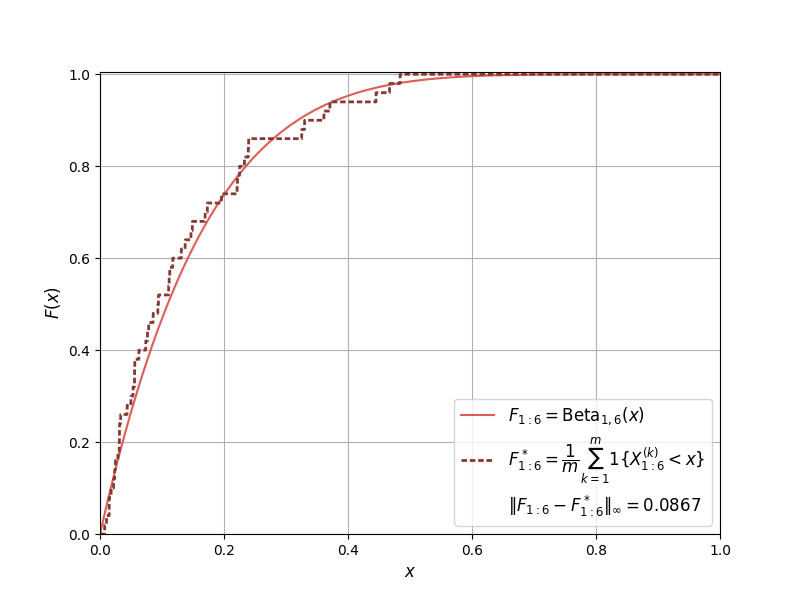
\includegraphics[trim={1.1cm 0.5cm 1.5cm 0cm}, clip,width=.46\linewidth]{../simulation/unif_order_1:6.png} \\
        $i = 1$
      \end{tabular}
    \begin{tabular}{@{}c@{}}
        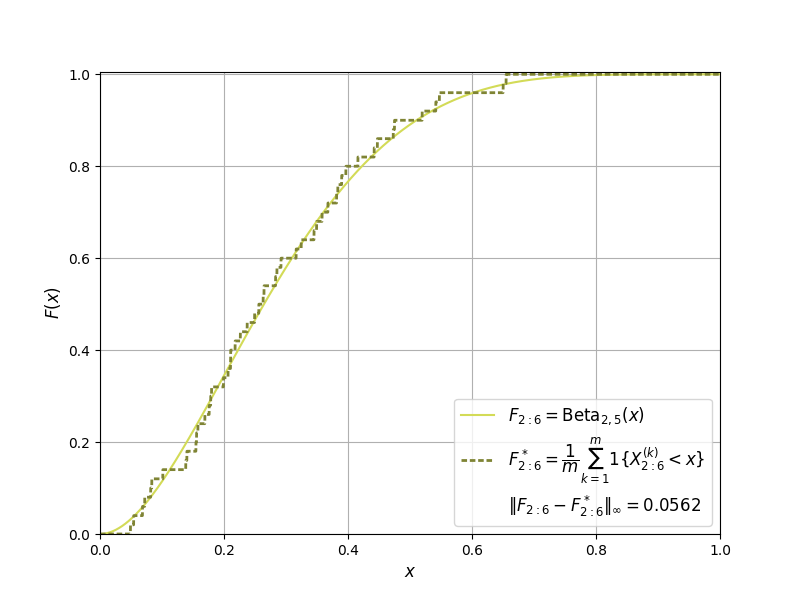
\includegraphics[trim={1.1cm 0.5cm 1.5cm 0cm}, clip,width=.46\linewidth]{../simulation/unif_order_2:6.png} \\
        $i = 2$
    \end{tabular}
    \begin{tabular}{@{}c@{}}
        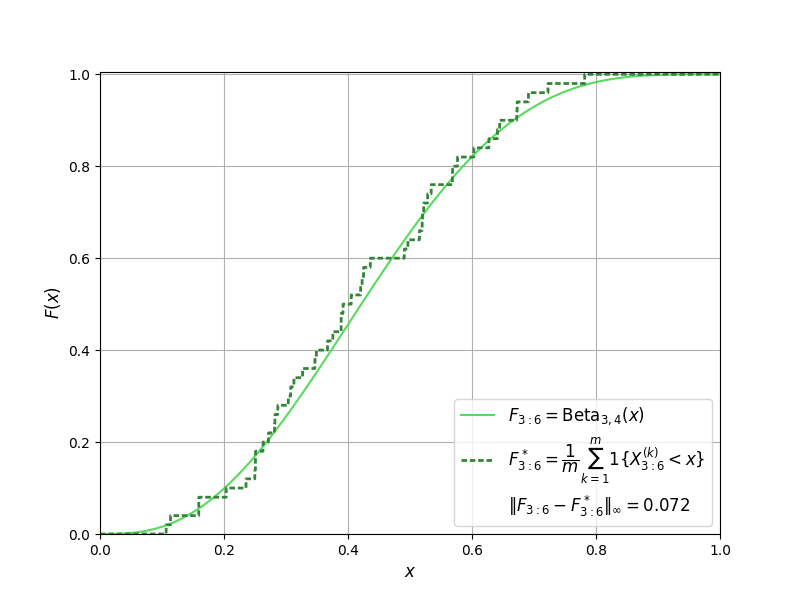
\includegraphics[trim={1.1cm 0.5cm 1.5cm 0cm}, clip,width=.46\linewidth]{../simulation/unif_order_3:6.png} \\
        $i = 3$
      \end{tabular}
    \begin{tabular}{@{}c@{}}
        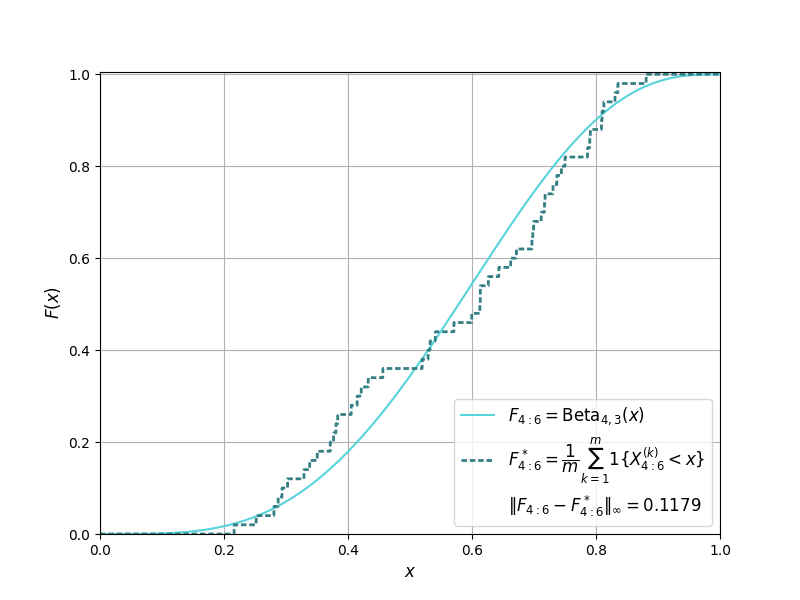
\includegraphics[trim={1.1cm 0.5cm 1.5cm 0cm}, clip,width=.46\linewidth]{../simulation/unif_order_4:6.png} \\
        $i = 4$
    \end{tabular}
    \begin{tabular}{@{}c@{}}
        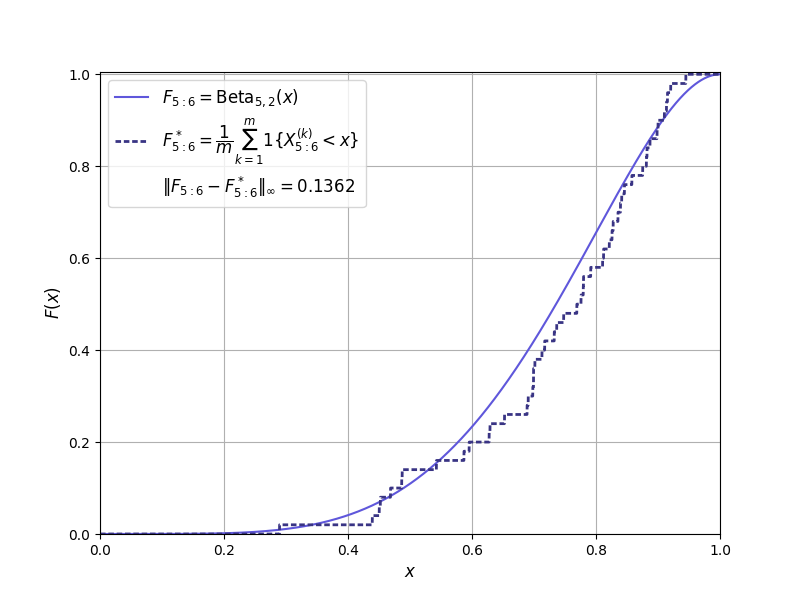
\includegraphics[trim={1.1cm 0.5cm 1.5cm 0cm}, clip,width=.46\linewidth]{../simulation/unif_order_5:6.png} \\
        $i = 5$
      \end{tabular}
    \begin{tabular}{@{}c@{}}
        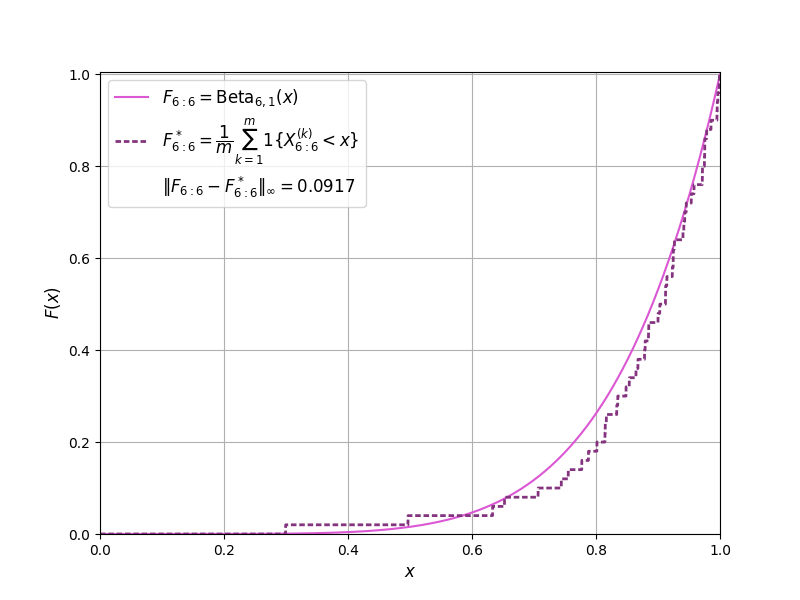
\includegraphics[trim={1.1cm 0.5cm 1.5cm 0cm}, clip,width=.46\linewidth]{../simulation/unif_order_6:6.png} \\
        $i = 6$
    \end{tabular}
    \caption{Simulation of the six order statistics for 6 samples of the Uniform Distribution}
\end{figure}

\newpage

\subsection*{Solution Part 2}

The distribution $F$ from part 2 is a type I Pareto distribution
\[ \text{Pareto}_{(\alpha, \sigma)}(x) = \begin{cases}
    0 & x\leq \sigma \\
    1- {\left( \frac{\sigma}{x} \right)}^{\alpha} & x > \sigma.
\end{cases} \]
with parameters $\alpha = \sigma = 1$. Therefore, the condition required for it to have the $k$-moment is that $k < \alpha$. Since $\alpha = 1$, it doesn't have any finite moments. Using the formula for the $i$-th statistic, we obtain
\[ F_{i:n}(x) = \sum_{j = i}^n \binom{n}{j} F^{j}(x)\ol{F}^{n-j}(x)\]
\[ = \sum_{j = i}^n \binom{n}{j} {(1-x^{-1})}^{j} x^{-n+j}. \]
Also,
\[ f_{i:n}(x) = \frac{1}{i}\cdot\binom{n}{i} f(x) F^{i-1}(x)\ol{F}^{n-i}(x) \]
\[ = \frac{1}{i}\cdot\binom{n}{i} x^{-2} {(1-x^{-1})}^{i-1}x^{i-n} \]
Thus, the formula for the $k$-moment is the following

\[ E[X^k] = \frac{1}{i}\cdot\binom{n}{i} \int_{1}^\infty \underbrace{x^{i+k} x^{-2-n}}_{\text{dominant}} {(1-x^{-1})}^{i-1} dx \]

This last integral converges if $n+2-i-k > 1$, thus, the only moments available are when $k < n-1-i$.

For the uniform norm I did the same as the previous part.

\newpage

\begin{figure}[H]
    \centering
    \begin{tabular}{@{}c@{}}
        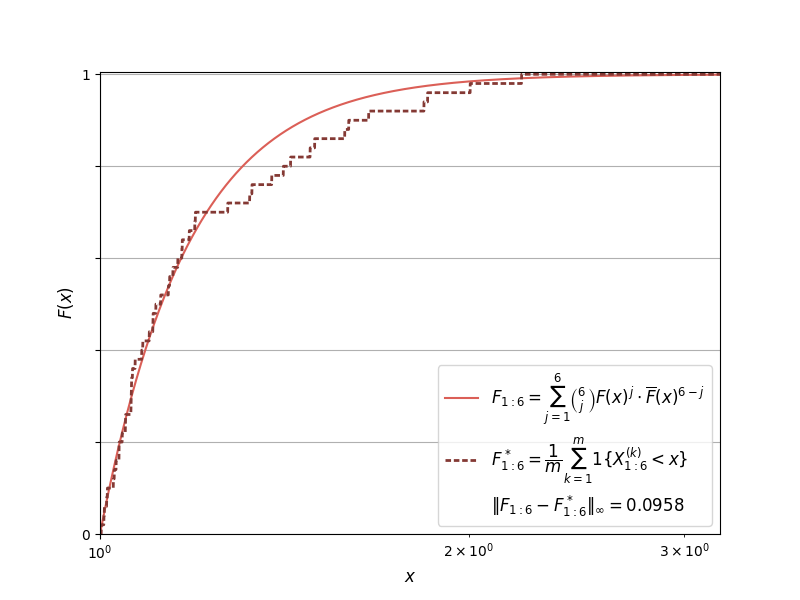
\includegraphics[trim={1.1cm 0.5cm 1.5cm 0cm}, clip,width=.46\linewidth]{../simulation/pareto_order_1:6.png} \\
        $i = 1$
      \end{tabular}
    \begin{tabular}{@{}c@{}}
        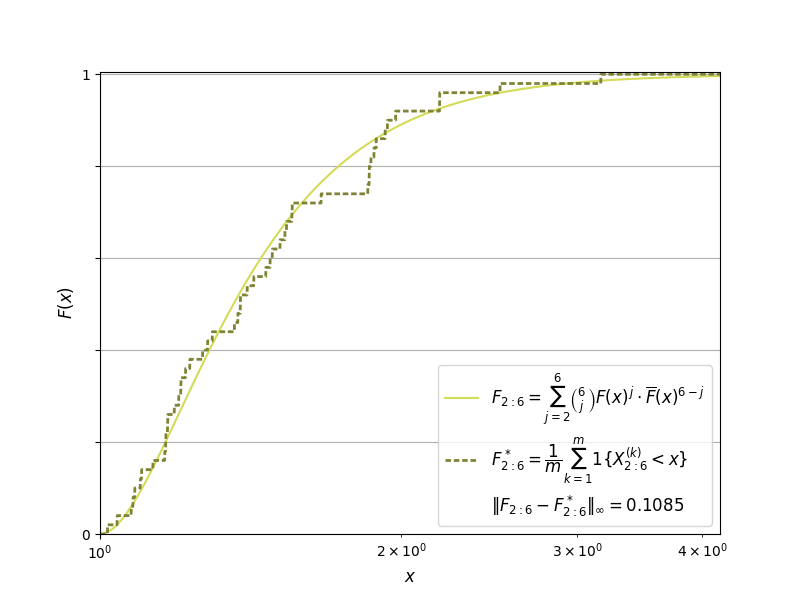
\includegraphics[trim={1.1cm 0.5cm 1.5cm 0cm}, clip,width=.46\linewidth]{../simulation/pareto_order_2:6.png} \\
        $i = 2$
    \end{tabular}
    \begin{tabular}{@{}c@{}}
        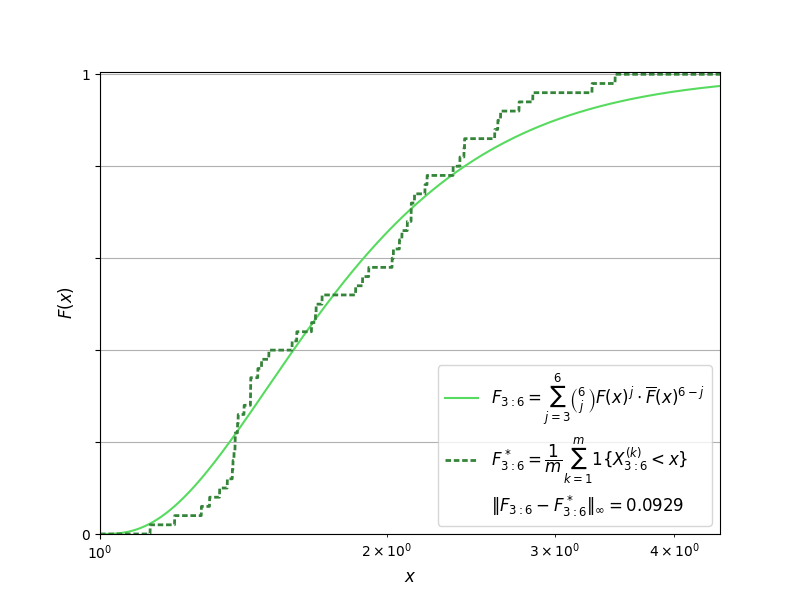
\includegraphics[trim={1.1cm 0.5cm 1.5cm 0cm}, clip,width=.46\linewidth]{../simulation/pareto_order_3:6.png} \\
        $i = 3$
      \end{tabular}
    \begin{tabular}{@{}c@{}}
        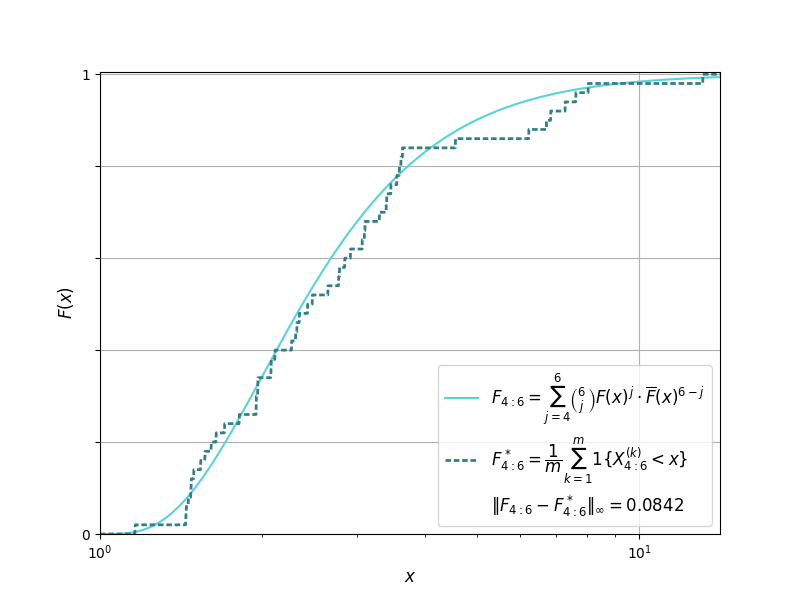
\includegraphics[trim={1.1cm 0.5cm 1.5cm 0cm}, clip,width=.46\linewidth]{../simulation/pareto_order_4:6.png} \\
        $i = 4$
    \end{tabular}
    \begin{tabular}{@{}c@{}}
        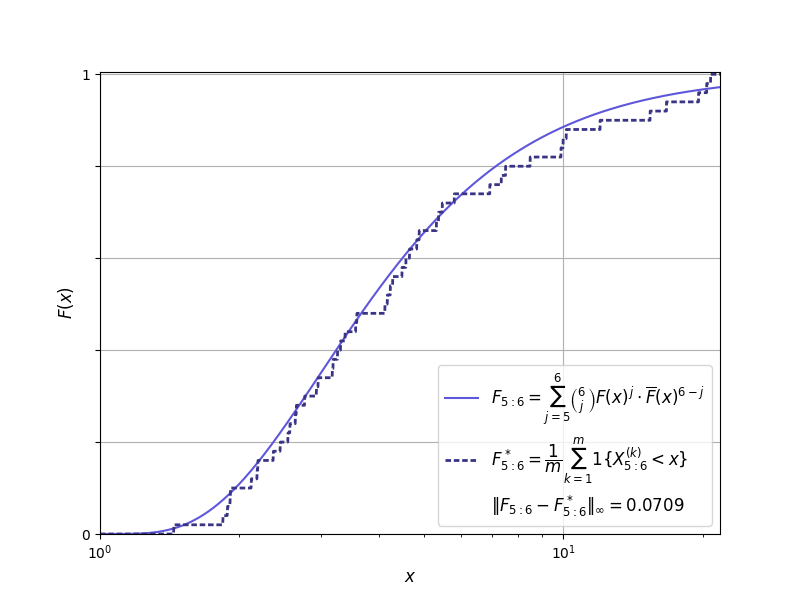
\includegraphics[trim={1.1cm 0.5cm 1.5cm 0cm}, clip,width=.46\linewidth]{../simulation/pareto_order_5:6.png} \\
        $i = 5$
      \end{tabular}
    \begin{tabular}{@{}c@{}}
        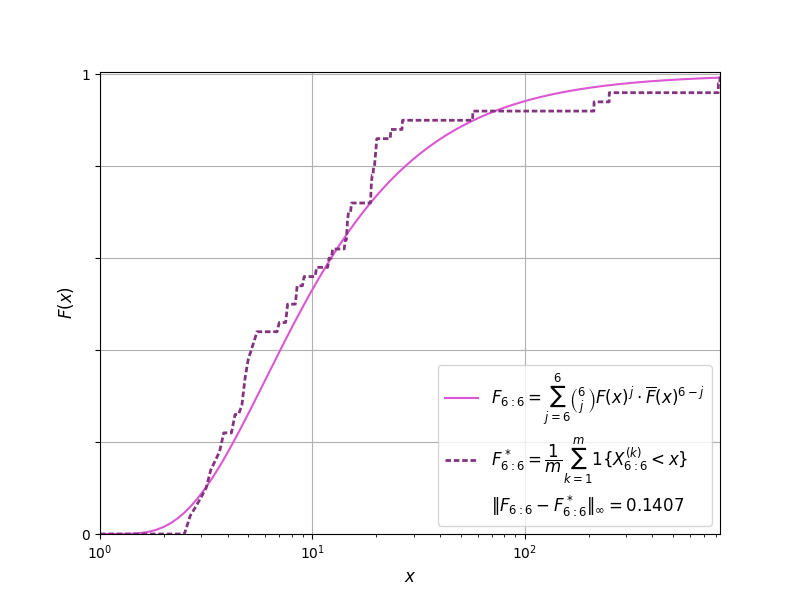
\includegraphics[trim={1.1cm 0.5cm 1.5cm 0cm}, clip,width=.46\linewidth]{../simulation/pareto_order_6:6.png} \\
        $i = 6$
    \end{tabular}
    \caption{Simulation of the six order statistics for 6 samples of the Pareto Distribution}
\end{figure}